%\chapres{\lipsum[1]}{\lipsum[2]}
\begin{figure}
    \centering
  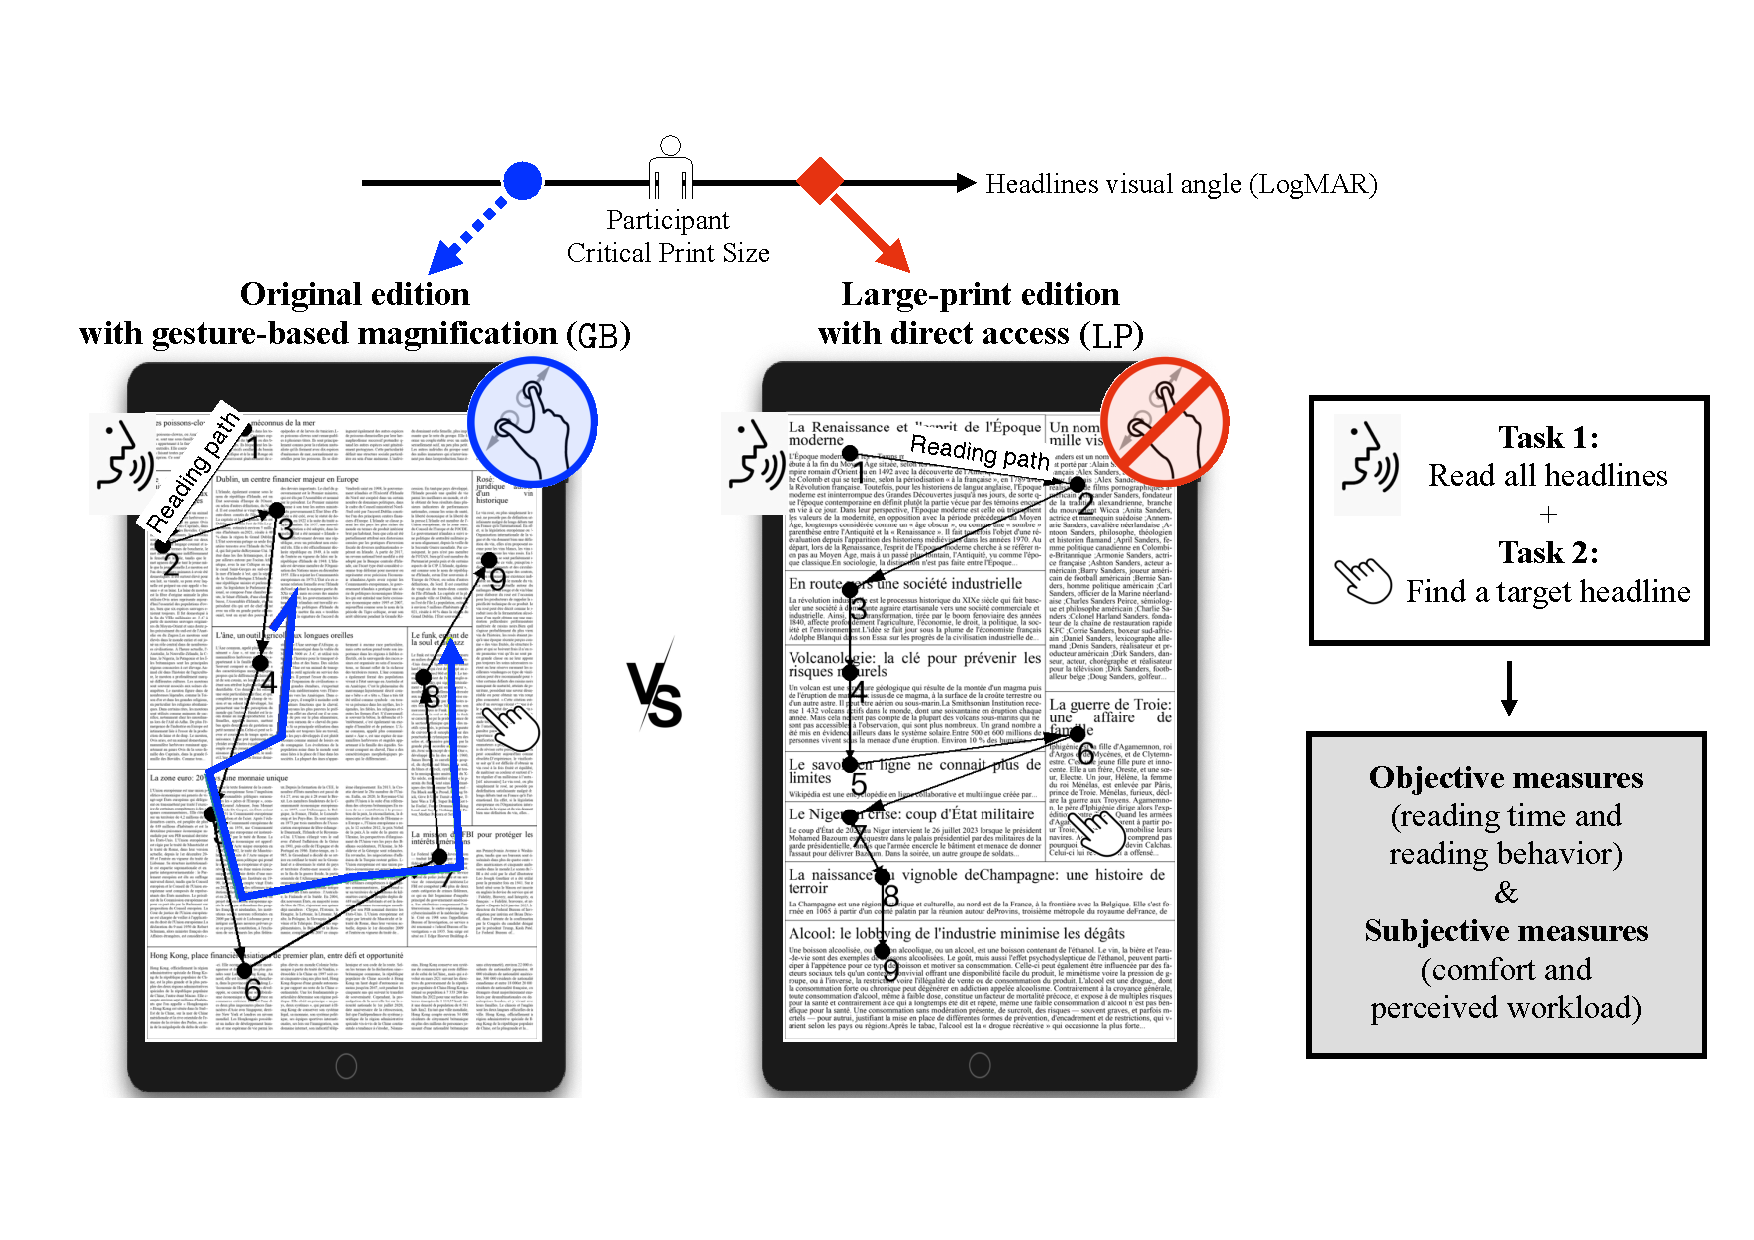
\includegraphics[width=0.8\columnwidth]{img/teaser.pdf}
  \caption{ Experimental protocol for quantifying the behavioral and performance cost of digital newspaper consumption under visual constraints. The figure illustrates the two conditions used to evaluate the impact of manual navigation versus direct structural access when reading digital newspapers. In the gesture-based magnification condition (\condonenot), participants read the original layout, in which headlines were rendered below each individual's Critical Print Size (CPS), requiring pan-and-zoom magnification (high manual control, fragmented global view). In the large-print edition with direct access condition (\condtwonot), headlines were enlarged above CPS and directly legible without magnification (no manual control, direct structural awareness). 
  Across multiple trials, participants performed two tasks—reading all headlines aloud and locating target articles—while both objective performance and subjective responses were collected.
  }
  \label{fig:teaser}
\end{figure}


\chaptoc